\documentclass[a4paper,11pt]{article}
\usepackage{amsmath,amsthm,amsfonts,amssymb,amscd,amstext,vmargin,graphics,graphicx,tabularx,multicol} 
\usepackage[francais]{babel}
\usepackage[utf8]{inputenc}  
\usepackage[T1]{fontenc} 
\usepackage{pstricks-add,tikz,tkz-tab,variations}
\usepackage[autolanguage,np]{numprint} 

\setmarginsrb{1.5cm}{0.5cm}{1cm}{0.5cm}{0cm}{0cm}{0cm}{0cm} %Gauche, haut, droite, haut
\newcounter{numexo}
\newcommand{\exo}[1]{\stepcounter{numexo}\noindent{\bf Exercice~\thenumexo} : \marginpar{\hfill /#1}}
\reversemarginpar


\newcounter{enumtabi}
\newcounter{enumtaba}
\newcommand{\q}{\stepcounter{enumtabi} \theenumtabi.  }
\newcommand{\qa}{\stepcounter{enumtaba} (\alph{enumtaba}) }
\newcommand{\initq}{\setcounter{enumtabi}{0}}
\newcommand{\initqa}{\setcounter{enumtaba}{0}}

\newcommand{\be}{\begin{enumerate}}
\newcommand{\ee}{\end{enumerate}}
\newcommand{\bi}{\begin{itemize}}
\newcommand{\ei}{\end{itemize}}
\newcommand{\bp}{\begin{pspicture*}}
\newcommand{\ep}{\end{pspicture*}}
\newcommand{\bt}{\begin{tabular}}
\newcommand{\et}{\end{tabular}}
\renewcommand{\tabularxcolumn}[1]{>{\centering}m{#1}} %(colonne m{} centrée, au lieu de p par défault) 
\newcommand{\tnl}{\tabularnewline}

\newcommand{\bmul}[1]{\begin{multicols}{#1}}
\newcommand{\emul}{\end{multicols}}

\newcommand{\trait}{\noindent \rule{\linewidth}{0.2mm}}
\newcommand{\hs}[1]{\hspace{#1}}
\newcommand{\vs}[1]{\vspace{#1}}

\newcommand{\N}{\mathbb{N}}
\newcommand{\Z}{\mathbb{Z}}
\newcommand{\R}{\mathbb{R}}
\newcommand{\C}{\mathbb{C}}
\newcommand{\Dcal}{\mathcal{D}}
\newcommand{\Ccal}{\mathcal{C}}
\newcommand{\mc}{\mathcal}

\newcommand{\vect}[1]{\overrightarrow{#1}}
\newcommand{\ds}{\displaystyle}
\newcommand{\eq}{\quad \Leftrightarrow \quad}
\newcommand{\vecti}{\vec{\imath}}
\newcommand{\vectj}{\vec{\jmath}}
\newcommand{\Oij}{(O;\vec{\imath}, \vec{\jmath})}
\newcommand{\OIJ}{(O;I,J)}


\newcommand{\reponse}[1][1]{%
\multido{}{#1}{\makebox[\linewidth]{\rule[0pt]{0pt}{20pt}\dotfill}
}}

\newcommand{\titre}[5] 
% #1: titre #2: haut gauche #3: bas gauche #4: haut droite #5: bas droite
{
\noindent #2 \hfill #4 \\
#3 \hfill #5

\vspace{-1.6cm}

\begin{center}\rule{6cm}{0.5mm}\end{center}
\vspace{0.2cm}
\begin{center}{\large{\textbf{#1}}}\end{center}
\begin{center}\rule{6cm}{0.5mm}\end{center}
}



\begin{document}
\pagestyle{empty}
\titre{Interrogation: Divisions décimales}{Nom :}{Prénom :}{Classe}{Date}


\exo{1.5} Poser et donner \textbf{la valeur exacte} des divisions suivantes :
\bmul{2}

\qa 393 $\div$ 16


\columnbreak


\qa $625,74 \div 8$



\emul

\vspace*{5cm}

\exo{2.5} Poser et donner \textbf{la valeur approchée} au millième près des divisions suivantes :

\bmul{3}

\initqa \qa  $127 \div 7$ 


\columnbreak


\qa $904,3 \div 6$

\columnbreak

\qa $25,84 \div 1,2$

\emul

\vspace*{6cm}

\exo{3} Compléter les calculs suivants :\\

\bmul{3}

$51,3 \div 100 =$\\

$. . . . . . . \div 10 = 58,74$\\

\columnbreak

$7  \div 10 =$

$5 847 \div . . . . . . . = 58,47$\\

\columnbreak

$28 \div 1 000 = $\\

$. . . . . . . \div 100 = 3,7$\\


\emul

\vspace*{1cm}


\exo{3} Voici les tarifs pour le mensuel Mepmagazine :\\

- en kiosque, il coûte 99 euros pour un an (soit 12 magazines) ;\\

- en prenant un abonnement, les 12 numéros coûtent 63 euros et les 24 numéros coûtent 114 euros.\\

\q Donner le prix d'un magazine si on l'achète en kiosque.\\
 \reponse[4]\\
 
 \newpage

\vspace*{0.5cm}

\q Donner le prix d'un magazine si on s'abonne pour 12 numéros.\\
 \reponse[3]\\

\q Donner le prix d'un magazine si on s'abonne pour 24 numéros.\\
 \reponse[3]\\
 
\q Quelle est la solution la plus avantageuse?\\
 \reponse[2]\\
 
 \vspace*{1cm}

\exo{} Bonus\\

\begin{center}
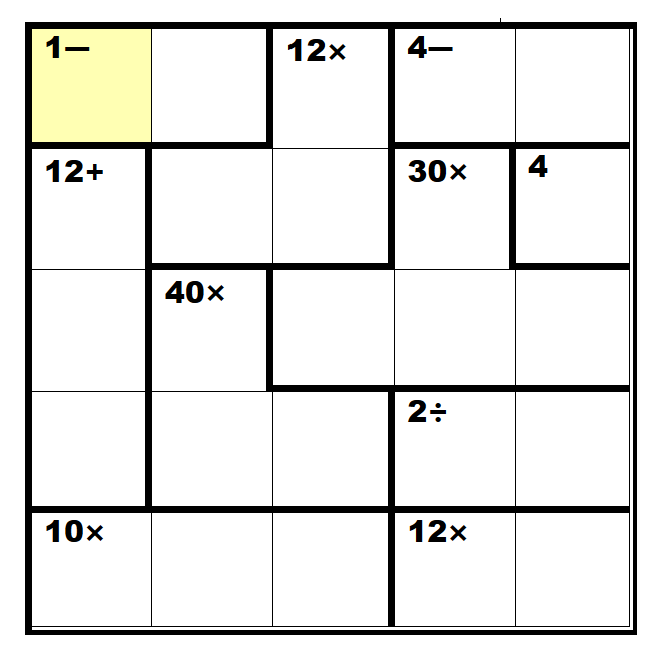
\includegraphics[scale=0.8]{kenken.eps} 

\end{center}


\end{document}
